\chapter{背景}\label{chap:background}

\section{特定脑区的重建}\label{sec:brain-region-reconstruction}
在脑类器官的研究中,重建特定脑区是一个重要的研究方向\cite{Kim2023}。
已有大量研究专注于如何通过干细胞技术培养出特定脑区的类器官。
例如,海马体、前额叶皮层和小脑等区域的重建已经取得了显著进展。
这些研究为脑类器官的功能研究提供了重要的基础。

\begin{figure}[!htbp]
    \centering
    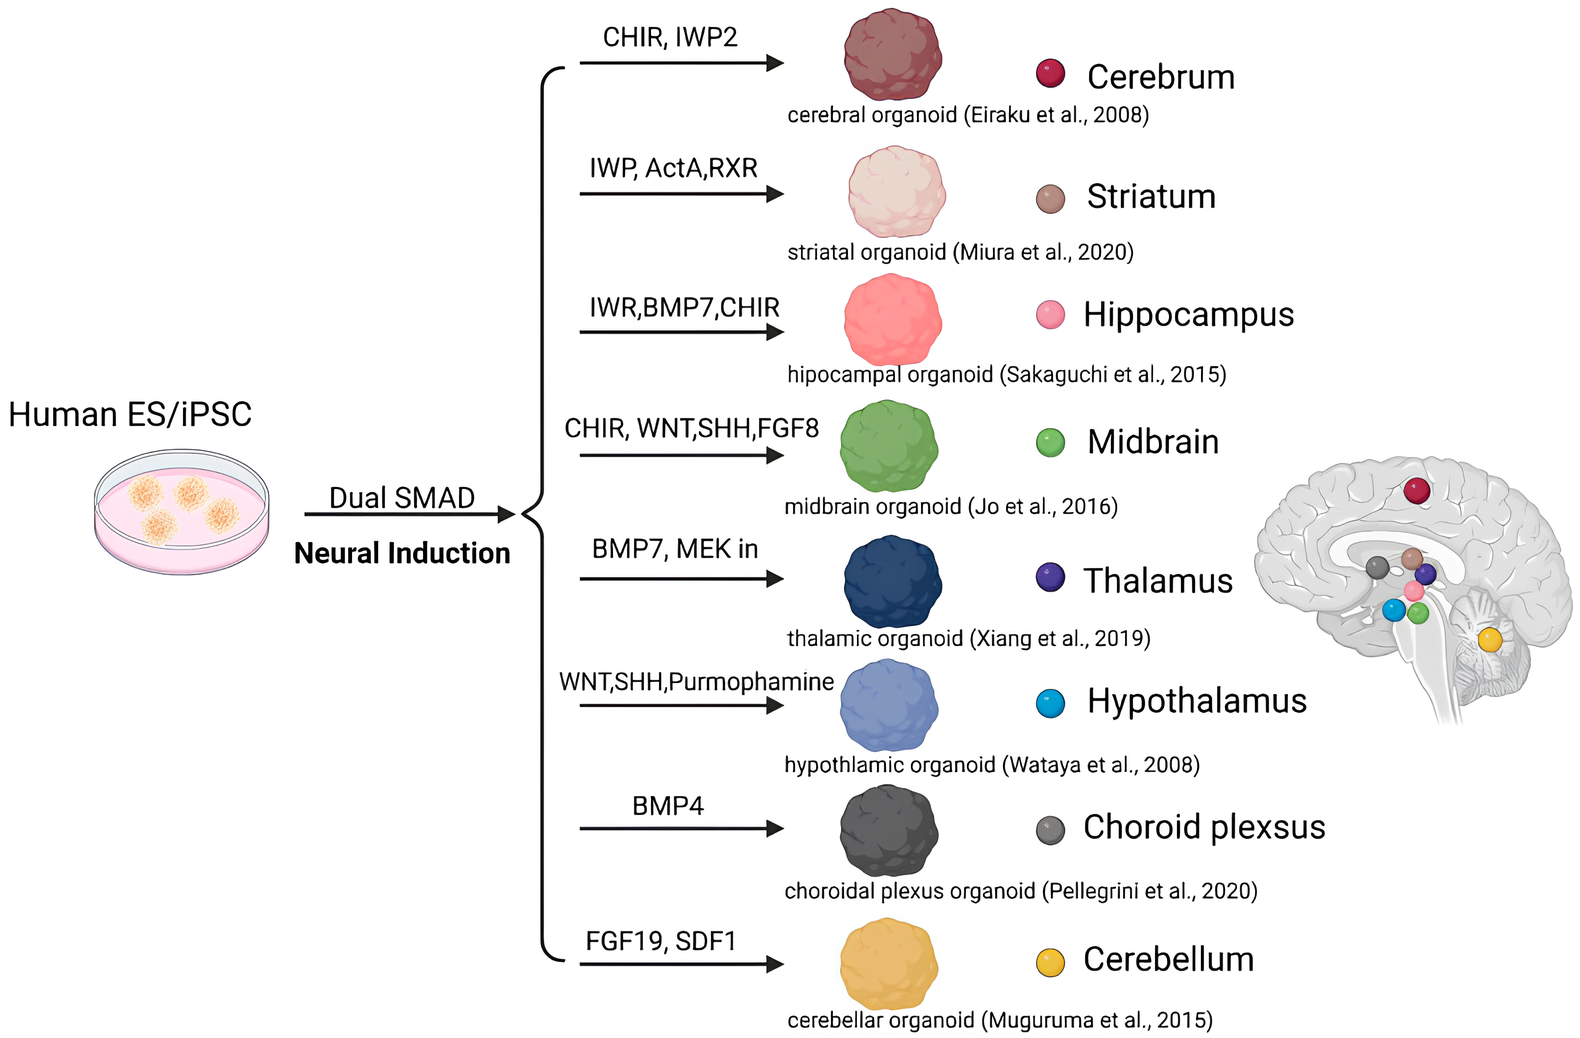
\includegraphics[width=0.75\textwidth]{Img/brain-organoids-regisons.png}
    \bicaption{经典脑区重建的研究现状\cite{Kim2023}}{Research Status of Classic Brain Region Reconstruction}
    \label{fig:brain-organoids-regisons}
\end{figure}

\section{自由能原理}\label{sec:free-energy-principle}
自由能原理(Free Energy Principle, FEP)是由 Karl Friston 于 2010 年提出的一种关于生命体智能的规范性理论\cite{Friston2010}。
该理论基于变分贝叶斯推断,认为生命体通过最小化自由能,即“惊奇”(Surprise),来维持其内部状态与外部环境的一致性。
自由能原理为理解大脑如何通过学习和适应来应对外部环境提供了理论框架。

\begin{figure}[!htbp]
    \centering
    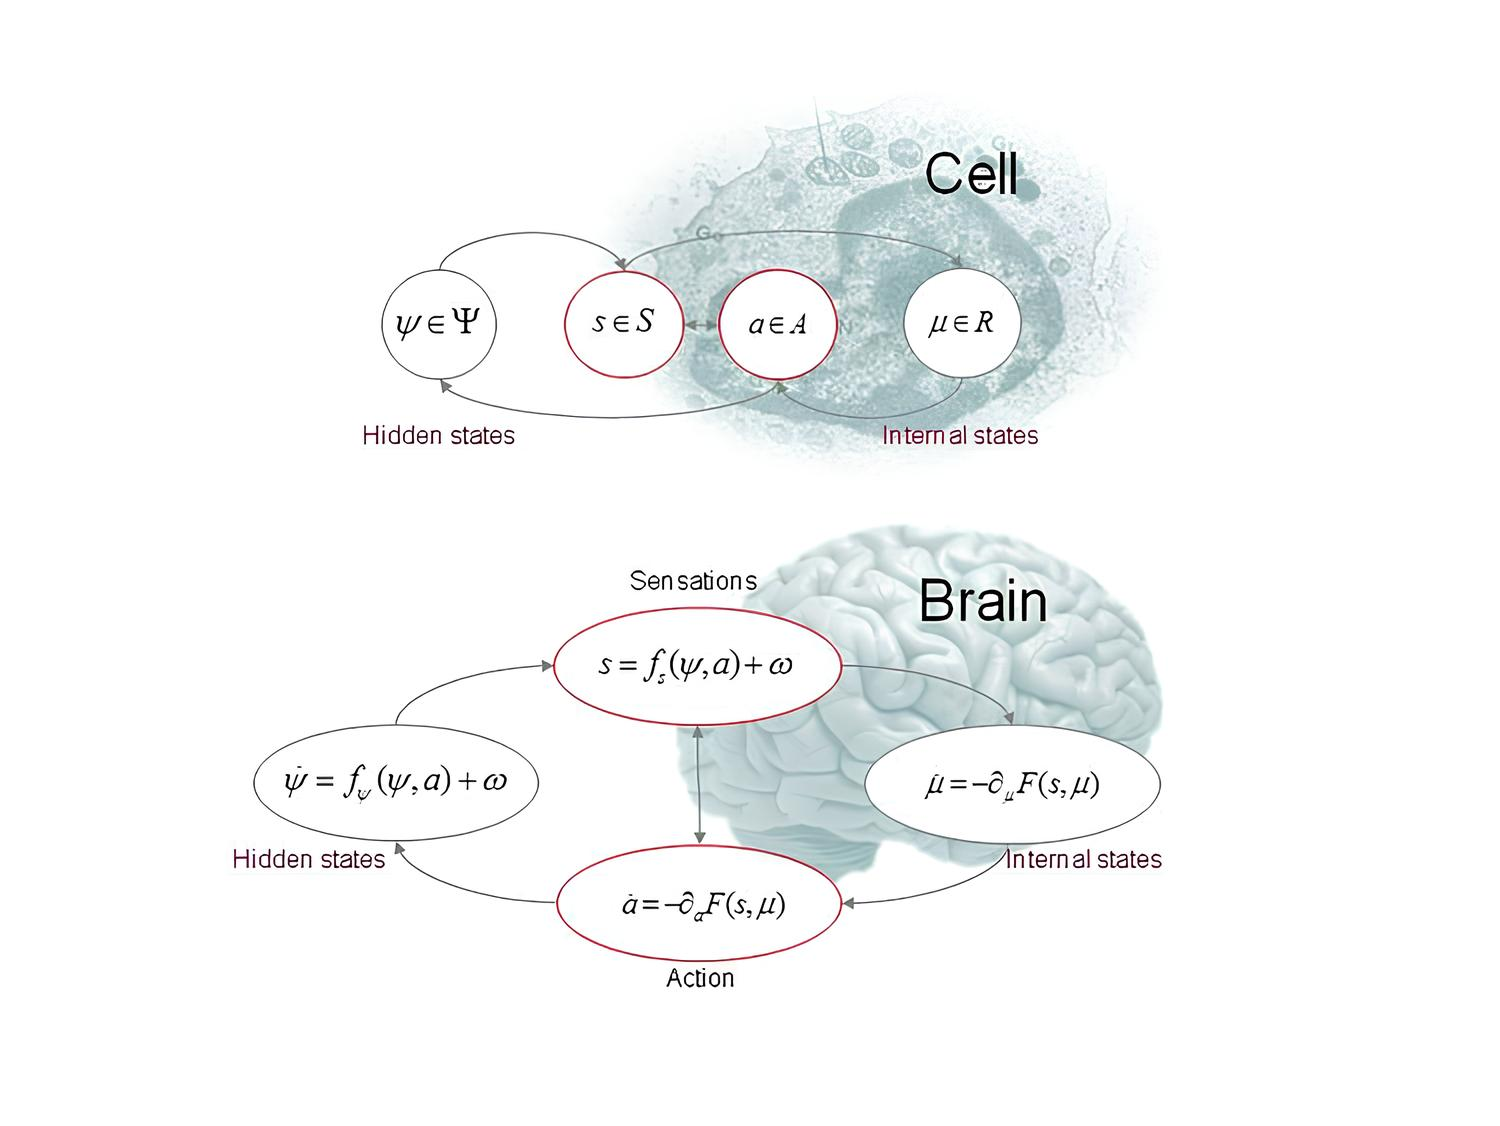
\includegraphics[width=0.75\textwidth]{Img/fep-marokov-blanket.jpg}
    \bicaption{马尔科夫毯与自由能原理\cite{wiki:free_energy_principle}}{Markov Blanket and Free Energy Principle}
    \label{fig:fep-marokov-blanket}
\end{figure}

\section{自由能原理的数学表达}\label{sec:free-energy-math}
自由能原理的核心思想可以通过以下数学公式表达:

\[
    \begin{aligned}
        \underbrace{F(\mu, a; s)}_{\text{free-energy}} & = \underbrace{\mathbb{E}_{q(\psi)} \left[ -\log p(\psi, s, a, \mu \mid \psi) \right]}_{\text{expected energy}} - \underbrace{\mathcal{H}[q(\psi \mid s, a, \mu, \psi)]}_{\text{entropy}} \\
                                                       & = \underbrace{-\log p(s)}_{\text{surprise}} + \underbrace{\text{KL}[q(\psi \mid s, a, \mu, \psi) \parallel p_{\text{Bayes}}(\psi \mid s, a, \mu, \psi)]}_{\text{divergence}}             \\
                                                       & \geq \underbrace{-\log p(s)}_{\text{surprise}}
    \end{aligned}
\]

其中,$F(\mu, a; s)$ 表示自由能,$\mathbb{E}_{q(\psi)}$ 表示期望能量,$\mathcal{H}$ 表示熵。
自由能原理认为,大脑通过变分贝叶斯推断来最小化自由能,从而使其对外部环境的预测尽可能准确。


\section{盘中之脑}\label{sec:dish-brain}
自由能原理不仅在理论上具有重要意义,还在实际研究中得到了广泛应用。
例如,基于自由能原理的“盘中之脑”(Dish Brain)项目成功训练了一个神经网络来玩电子游戏\cite{Kagan2022}。
这一研究表明,通过外部刺激和奖励机制,可以在体外培养出具有学习能力的神经网络。

\begin{figure}[!htbp]
    \centering
    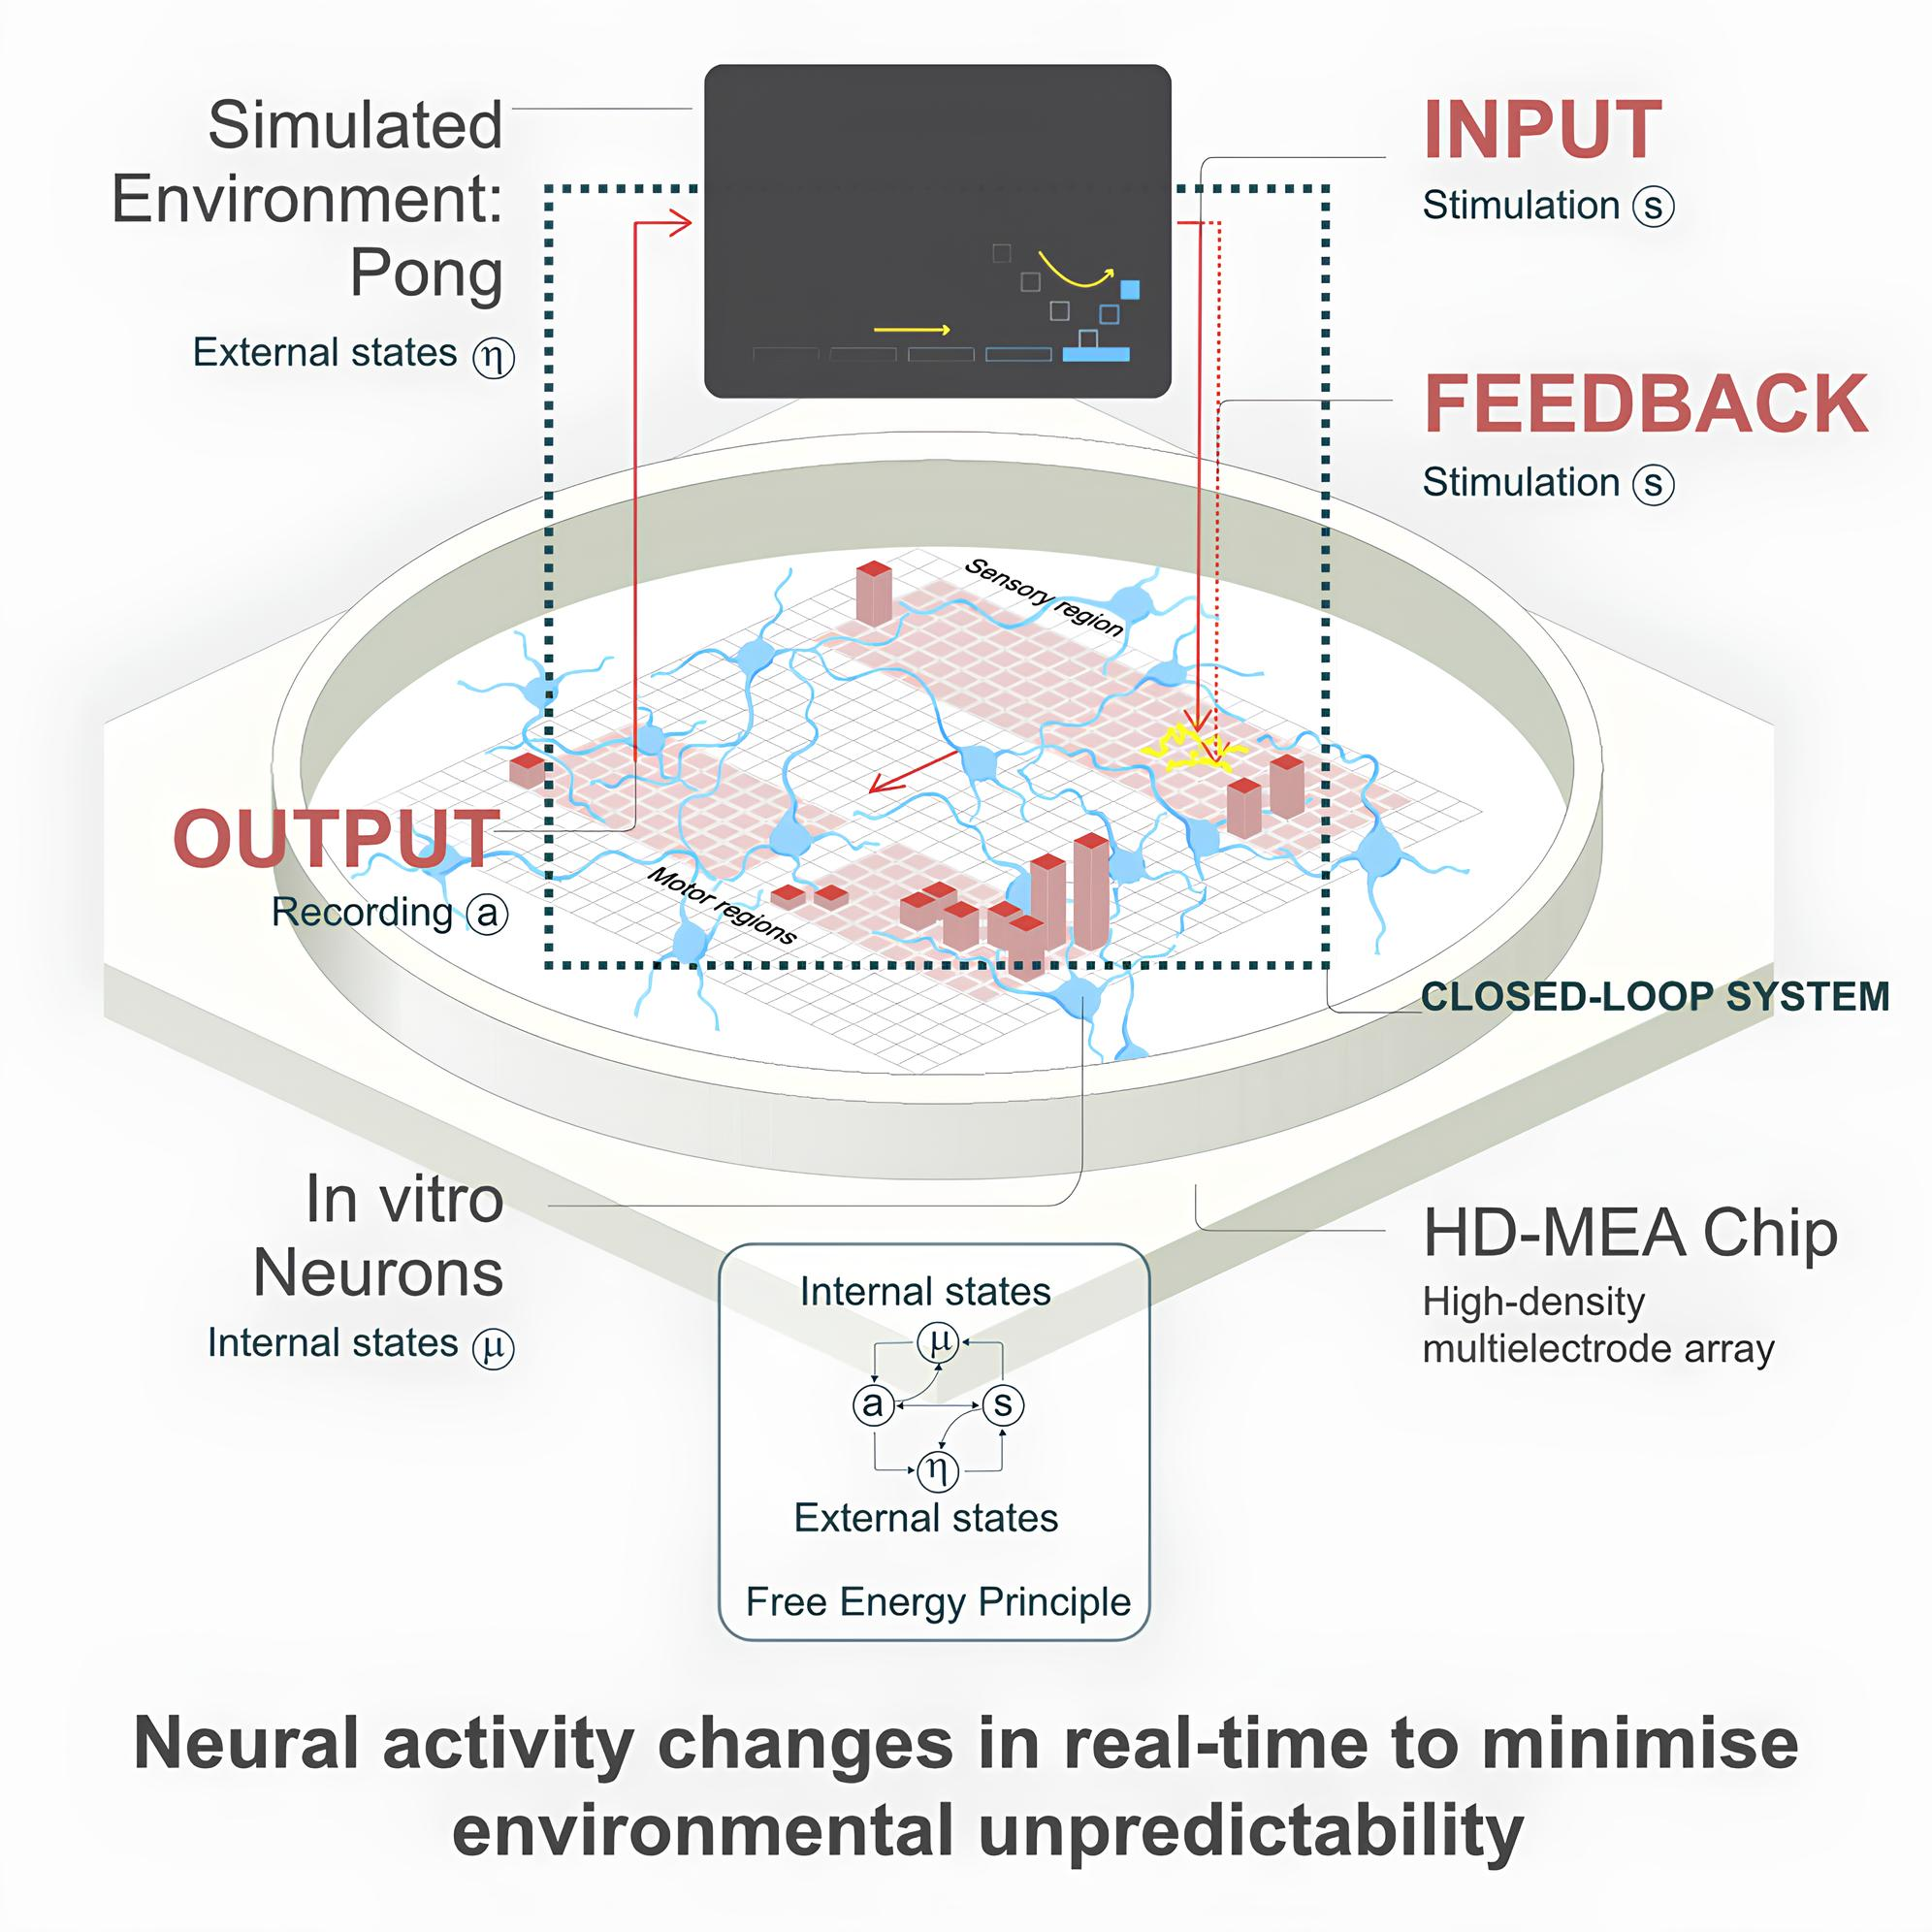
\includegraphics[width=0.75\textwidth]{Img/dishbrain-absract.jpg}
    \bicaption{盘中之脑的图片摘要\cite{Kagan2022}}{Abstract Diagram of Dish Brain}
    \label{fig:dishbrain-absract}
\end{figure}
